% mainfile: ../../Refinement.tex
The \findex[\picalc{}|(]{\picalc{}} is a process algebra that can be used to describe the behavior. This section introduces the pure polyadic version of the \picalc{} as decriped in \cite{milner}. 


\subsection{Intuition}
\label{sec_pi_intuition}
% mainfile: ../../Refinement.tex
To explain the \picalc{} inuitivly we will use the ion example as in \cite{milner}. Let us imagine a positive and a negative ion. When those two ions merge, we get a new construct. The merge operation is called a reaction, since an ion acts and the other reacts. This reaction can be seen as communication between two processes. The two processes communicate to share some information.  One process is the sender and the other is the receiver. By doing the reaction both processes evoulte to some thing new. The reaction, information sharing and evolution concepts are the core of the \picalc{}. Using those concepts we can understand the title of Milner's book \textit{communicating and mobile processes}: the \picalc{} \cite{milner}. The word \textit{communicating} refers to the \textit{reaction} concept. The word \textit{mobile} refers to the \textit{information sharing and evolution} concepts, since the receiver process can use the received information to change its location as we will see in \refSec{sec_pi_mobility}.
\\Intuitively, the \picalc{} consists of: 
\begin{itemize}
\item a set of names starting with capital case letters  like $P, P_1, Q,..etc$  used to refer to a process directly.
\item a set of names starting with capital case letters  like $A, B, C,..etc$  used a process identifier. The process identifier will be used to define recursion with parameters.
\item a set of names starting with lower case letter like $a, b, x, y,..etc$  used as a channel and message name. This set is denoted by $\names$.
\item operators like:
	\begin{itemize}
	\item  Parallel composition operator: `` $\procpar{}{}$ ''.
	\item  Sequential composition operator: `` $.$ ''.
	\item  Choice operator: `` $\procchoice{}{}$ ''.
	\item  Scope restriction operator: `` $\procres{}{}$ ''.
	\end{itemize}
\end{itemize}
So a simple example of a process can be: $\out{x}{y}.\proczero$ this process simply sends the message $y$ via the channel $x$ and stops.
The full syntax of \picalc{} process is given in \refDef{def_process_syntax}. In this thesis starting from this point, when we mention the word \textit{names} we refer to $\names$. Furthermore, we shall often write $\vec{y}$ for a \findex[sequence]{sequence} $y_1,....,y_n$ of names.


\subsection{Syntax}
\label{sec_pi_syntax}
% mainfile: ../../Refinement.tex
\begin{definition}[Process syntax]
\label{def_process_syntax}
The syntax of a \picalc{} process \findex[process]{P} is defined by: 
\begin{align*}
 P & \syntdef \procsum \ebnf \procpar{P_1}{P_2} \ebnf \procres{\vec{y}}{P} \ebnf \proccall{A}{\vec{v}}
\end{align*}
where:
\begin{itemize}
\item $\procsum$ is the guarded sum.
\item $\procpar{P_1}{P_2}$ is the parallel composition of processes.
\item $\procres{\vec{y}}{P}$ is the restriction of the scope of the names $\vec{y}$ to the process $P$
\item $\proccall{A}{\vec{v}}$ is a process call. 
\end{itemize}
\end{definition}

\subsubsection{\findex{Guarded sum}:} The guarded sum is the \findex{choice} between multiple guarded processes. If the guard of one process took place, other guarded processes will be discarded. For example, the processes: $\procchoice{\inp{x}{}.P_1}{\inp{y}{}.P_2}$ will evolve to the process $P_1$ if the guard $\inp{x}{}$ occurred.

Furthermore, The process $\proczero$ is called the \index{process!stop}\findex{stop process} or \findex{inaction} and stands for the process that can do nothing. It can be omitted.
\subsubsection{\findex{Guard}:} The guard is also called \findex[process]{action prefix} and denoted by $\pi$. It's syntax is defined by:
\begin{definition}[Action prefix syntax]
\label{def_prefix_syntax}
\begin{align*}
 \pi \syntdef \out{x}{\vec{y}} \ebnf \inp{x}{\vec{y}} \ebnf \tau
\end{align*}
where:
\begin{itemize}
\item $\out{x}{\vec{y}}$ \footnote{$\out{x}{{}}$ means: send a signal via $x$. $\out{x}{{y}}$ means: send the name $y$ via $x$.  $\out{x}{{\vec{y}}}$ means: send the sequence $\vec{y}$ via $x$.} represents the action: send $\vec{y}$ via the channel $x$.
\item $\inp{x}{\vec{y}}$ \footnote{$\inp{x}{{}}$ means: receive a signal via $x$. $\inp{x}{{y}}$ means: receive any name $y$ via $x$.  $\inp{x}{{\vec{y}}}$ means: receive any sequence $\vec{y}$ via $x$. ``$y$ here plays the role of parameter''} represents the action: receive $\vec{y}$ via the channel $x$.
\item $\tau$ represents an internal non observable action.
\end{itemize}
\end{definition}
The set of all \index{action}\findex[action]{actions} is defined as $\actions\define\outA\cup\inA\cup\set{\tau}$, where:
\begin{itemize}
\item $\outA$ is the set of all \index{action!output}\findex[output!action]{output actions}, defined as $\outA\define\set[x\in\names]{\out{x}{\vec{y}}}$.
\item $\inA$ the set of all \index{action!input}\findex[input!action]{input actions}, defined as $\inA\define\set[x\in\names]{\inp{x}{\vec{y}}}$.
\end{itemize}
\subsubsection{\findex{Parallel composition}:}
The parallel composition operator $\procpar{}{}$ represents the concept of concurrency in the \picalc{}, where two processes can evolve in concurrent.It represents an interleaving behavior of the concurrency.
For example let:  $P\define\procpar{P_1}{(\procpar{P_2}{P_3})}$ where: $P_1\define\inp{x}{y}.Q_1$ , $P_2\define\out{x}{y}.Q_2$ and $P_3\define\inp{x}{y}.Q_3$. So $P\define\procpar{\inp{x}{y}.Q_1}{(\procpar{\out{x}{y}.Q_2}{\inp{x}{y}.Q_3})}$.
Possible evolution cases of $P$ are:
\begin{itemize}
\item $\procpar{P_1}{(\procpar{Q_2}{Q_3})}$. $P_2$ sends $y$ via $x$ to $P_3$.
\item $\procpar{Q_1}{(\procpar{Q_2}{P_3})}$. $P_2$ sends $y$ via $x$ to $P_1$.
\end{itemize}

The example above illustrated the privacy nature of the parallel operator in the \picalc{}. A process can via a channel communicate with only one process pro time, i.e., the channel represents a binary synchronization. $P_2$ cannot communicate with both $P_1$, $P_3$ in the same time, while in \gls{CSP} a process can communicate with multiple processes in the same time via the same channel by sending multiple copies of the same message, i.e., in CSP the channel represents a multiple synchronization.


\subsubsection{\findex{Restriction}:}

The expression $\procres{\vec{y}}{P}$ binds the names $\vec{y}$ to the process $P$. In other words: the visibility scope of the  names $\vec{y}$ is restricted to the process $P$. It is similar to declaring a private variable in programming languages. Thus the names $\vec{y}$ are not visible outside $P$ and $P$ cannot use them to communicate with outside. For example, let $P\define\procpar{P_1}{P_2}$ where: $P_1\define\procres{y}{\out{y}{z}.Q_1}$ and $P_2\define\inp{y}{z}.Q_2$. The process $P$ cannot evolute to $\procpar{Q_1}{Q_2}$, since the name $y$ in $P_1$ is only visible inside it, i.e., from the $P_2$'s point of view $P_1$ doesn't have a channel called $y$. This takes us to the definition of the Bound and free names.

\begin{definition}[Free names]
\label{def_bound_names}
 are all the restricted names in a process.
\end{definition}
\begin{definition}[Bound names]
\label{def_free_names}
 are all the name that occur in a process except the bound names.
\end{definition}

For example, let $P_1\define\procres{x}{\out{x}{y}.P_2}$ where $P_2\define\procres{z}{\out{x}{z}.P_3}$. The name $x$ is bound in $P_1$ but free in $P_2$.


\subsubsection{\findex{Process call}:}
\label{subsubsection_process_call}

Let $P$ be a process and let $A$ be a process identifier.To be able to use the process $P$ recursively we use the process identifier $A$ as follow: $\procdef{A}{\vec{w}}\define{}P$. Thus , when we write $\proccall{A}{\vec{v}}$ we are using the identifier $A$ to call the process $P$ with replacing the names $\vec{w}$ in $P$ with the names $\vec{v}$. This replacement is called the $\alpha$-conversion

For example, let $P\define\out{w}{y}.\proczero$ and let $\procdef{A}{w}\define{}P$ be the recursive definition of the process $P$, then the behavior of $\proccall{A}{v}$is equlivant to $\out{v}{y}.\proczero$ 



\subsection{Semantics}
\label{sec_pi_sem}
% mainfile: ../../Refinement.tex
To understand the operational semantics of \picalc{} we will use  a labelled transition system LTS. Using this LTS we can investigate \picalc{} process evolution. The definition of LTS is adapted from \cite{milner} pages 39\footnote{Transition Rules: LTS for concurrent processes not for \picalc{} processes.}, 91\footnote{Reaction Rules: no labels and no LTS.}, 132\footnote{Commitment Rules: abstractions and concretions are out of this thesis's scope.} with some changes.

\subsubsection{Definition}
\begin{definition}[The LTS of \picalc{}]
\label{def_trans_system}

The labelled transition system $(\procs,\traces)$ of \picalc{} processes over the action set $\actions$ has the process expressions $\procs$ as its states, and its transitions $\traces$ are those which can be inferred from the rules in \refFig{fig_transition_rules}.
The rule REACT is the most important one. It shows the process evolution when a reaction occurs. The reaction requires two complementary transitions $P \transs{\out{x}{\vec{y}}} P'$ and $Q \transs{\inp{x}{\vec{z}}} Q'$, we call them commitments. so the process $P$ takes a commitment to take part in the reaction, and so does $Q$.
% mainfile: ../../Refinement.tex
\begin{figure}[H]
\begin{gather*}
\underline{\scriptstyle{OUT}}: \out{x}{\vec{y}}.P \transs{\out{x}{\vec{y}}} P
\quad\quad
\underline{\scriptstyle{IN}}: \inp{x}{\vec{y}}.P \transs{\inp{x}{\vec{y}}} P
\\\\
\underline{\scriptstyle{TAU}}: \tau.P \transs{\tau} P
\quad\quad
\underline{\scriptstyle{SUM}}: \procchoice{\alpha.P}{\procsum} \transs{\alpha} P
\\\\
\kalRule[]{L\_PAR}{}{P \transs{\alpha} P'}{\procpar{P}{Q} \transs{\alpha} \procpar{P'}{Q}}
\quad\quad
\kalRule[]{R\_PAR}{}{Q \transs{\alpha} Q'}{\procpar{P}{Q} \transs{\alpha} \procpar{P}{Q'}}
\\\\
\kalRule[if\ \alpha \nin \{\overline{x},x\}]{RESTRICTION}{}{P \transs{\alpha} P'}{\procres{x}{P} \transs{\alpha} \procres{x}{P'}}
\\\\
\kalRule[if\ \procdef{A}{\vec{z}}\define{}P]{PROCESS\_CALL}{}{\substitue{\vec{y}}{\vec{z}}P \transs{\alpha} P'}{\proccall{A}{\vec{y}} \transs{\alpha} P'}
\\\\
\kalRule[]{REACT}{P \transs{\out{x}{\vec{y}}} P'}{Q \transs{\inp{x}{\vec{z}}} Q'}{\procpar{P}{Q} \transs{\tau} \procpar{P'}{\substitue{\vec{y}}{\vec{z}}Q'}}
\end{gather*}
\caption{The \index{transition rules}\findex{transition rules} \cite{milner}.}
\label{fig_transition_rules}
\end{figure}


\end{definition}


An example of using the transition rules of this LTS to infer a transition: Let $P\define\procres{x}{(\procpar{\proccall{A}{x}}{\proccall{B}{x}})}$ where: $\procdef{A}{y}\define{}\out{y}{{}}.\proccall{A'}{y}$ and $\procdef{B}{z}\define{}\inp{z}{{}}.\proccall{B'}{z}$. the process $P$ can do the transition $\procres{x}{(\procpar{\proccall{A}{x}}{\proccall{B}{x}})} \transs{\tau} \procres{x}{(\procpar{\proccall{A'}{x}}{\proccall{B'}{x}})}$, which is a reaction.The inference tree of this transition is shown in \refFig{fig_inference_tree}. Thus, using the LTS we can enumerate sll possible transitions of a \picalc{} process.
% mainfile: ../../piOZ.tex
\begin{figure}[htbp]
\scalebox{0.93}{
\begin{prooftree} 
\infer0[by OUT]{\out{x}{{}}.\proccall{A_2}{x} \transs{\out{x}{{}}} \proccall{A_2}{x}}
\infer1[by PROCESS CALL]{\proccall{A_1}{x} \transs{\out{x}{{}}} \proccall{A_2}{x}}
\infer0[by IN]{\inp{x}{{}}.\proccall{B_2}{x} \transs{\inp{x}{{}}} \proccall{B_2}{x}}
\infer1[by PROCESS CALL]{\proccall{B_1}{x} \transs{\inp{x}{{}}} \proccall{B_2}{x}}
\infer2[by REACT]{ \procpar{\proccall{A_1}{x}}{\proccall{B_1}{x}} \transs{\tau} \procpar{\proccall{A_2}{x}}{\proccall{B_2}{x}} }
\infer1[by RESTRICTION]{ \procres{x}{(\procpar{\proccall{A_1}{x}}{\proccall{B_1}{x}})} \transs{\tau} \procres{x}{(\procpar{\proccall{A_2}{x}}{\proccall{B_2}{x}})} }                       
\end{prooftree}
}
\caption{The \index{inference tree}\findex{inference tree} \cite{milner}.}
\label{fig_inference_tree}
\end{figure}




\subsection{Visualization}
\label{sec_pi_visualization}
% mainfile: ../../Refinement.tex
To gain more understanding of the \picalc{} we will use \findex[stargazer]{Stargazer}\cite{stargazer}. Stargazer is a visual simulator for \picalc{}. \refLis{pi_visualization_stargazer_code} shows the code of the process $P\define\procres{x}{(\procpar{\proccall{A_1}{x}}{\proccall{B_1}{x}})}$ where: $\procdef{A_1}{y}\define{}\out{y}{{}}.\proccall{A_2}{y}$ and $\procdef{B_1}{z}\define{}\inp{z}{{}}.\proccall{B_2}{z}$ in stargazer syntax.
\lstinputlisting[backgroundcolor=\color{white},caption={stargazer code for the process $P$.},captionpos=b, label={pi_visualization_stargazer_code}]{listings/pi_visualization_stargazer.pi}
\raggedbottom

Stargazer can visualize the reaction $\procres{x}{(\procpar{\proccall{A_1}{x}}{\proccall{B_1}{x}})} \transs{\tau} \procres{x}{(\procpar{\proccall{A_2}{x}}{\proccall{B_2}{x}})}$ as shown in
\refFig{pi_visualization_stargazer_reaction}.

\begin{figure}[H]%
\centering
\subcaptionbox{Before reaction occurrence.}{\fbox{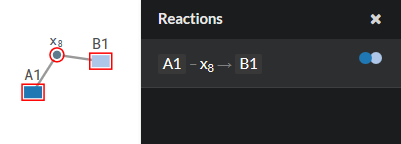
\includegraphics[width=0.45\textwidth]{./images/pi_visualization_stargazer_Before_react.png}}}%
\hfill
\subcaptionbox{After reaction occurrence.}{\fbox{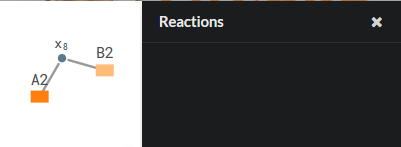
\includegraphics[width=0.45\textwidth]{./images/pi_visualization_stargazer_After_react.png}}}%
\caption{The process $P$ reaction}
\label{pi_visualization_stargazer_reaction}%
\end{figure}

\subsection{Simulation}
\label{sec_pi_simulation}
% mainfile: ../../Refinement.tex
The \findex[simulation!strong]{strong simulation} is a comparison of processes based on their behavior. To understand this let us start with a simple example:
Let $P\define\tau.\tau.\proczero$ and $Q\define\tau.\proczero$. We can notice that $P$ can do two $\tau$ transitions, but $Q$ can do only one. Thus $Q$ does not strongly simulates $P$. The word \textit{strongly} refers to the point that: the strong simulation comparison takes the internal transition $\tau$ into account. There is another kind of comparison called the  \findex[simulation!weak]{weak simulation}, which does not consider the internal transition $\tau$, but this kind of comparison is not considered in this thesis. The formal definition of the strong simulation is given in \refDef{def_strong_sim}.

\begin{definition}[Strong simulation]
\label{def_strong_sim}
A relation $\mathcal{S}\subseteq\procs\times\procs$ is called a \findex[simulation!strong]{strong simulation}, if $(P,Q)\in\mathcal{S}$ implies that
\[\text{if } P \transs{\alpha} P' \text{ then }Q'\in\procs \text{ exists such that } Q \transs{\alpha} Q' \text{ and } (P',Q')\in\mathcal{S}.\]
where $\alpha$ is an input, output or $\tau$ action.
\end{definition}

An example of checking the strong simulation is:
\\Let
\begin{itemize}
\item $P\define\procres{x}{(\procpar{\proccall{A_1}{x}}{\proccall{B_1}{x}})}$ 
\item $Q\define\procres{x}{(\procchoice{(\procpar{\proccall{A_1}{x}}{\proccall{B_1}{x}})}{\tau.Q})}$
\end{itemize}
where:
\begin{itemize}
\item $\procdef{A_1}{y}\define{}\out{y}{{}}.\proczero$
\item $\procdef{B_1}{z}\define{}\inp{z}{{}}.\proczero$
\end{itemize}

Intuitively, The behavior of $P$ and $Q$ can be illustrated using transition graphs as shown in \refFig{transition_graphs}. $Q$'s transition graph is the same as $P$'s, except one thing: $Q$ has a loop with label $\tau$. This loop is due to the $\tau$ transition in $Q$'s definition. Hence, we can notice that $Q$ can do all the transitions that $P$ can, plus an extra transition $\tau$. In other words $Q$ simulates $P$, but $P$ doesn't simulate $Q$.
\begin{figure}[H]%
    \centering
    \subfloat[$P$]{{\fcolorbox{black}{white}{
    \begin{tikzpicture}[->,>=stealth',shorten >=1pt,auto,node distance=3cm,
                    semithick]
  \tikzstyle{every state}=[]

  \node[state] (A)                    {$\procres{x}{(\procpar{\out{x}{}.\proczero}{\inp{x}{}.\proczero})}$};
  \node[state]         (B) [right of=A] {$\proczero$};
  \path (A) edge              node {$\tau$} (B);
\end{tikzpicture}
 }}}%
    \qquad
    \subfloat[$Q$]{{\fcolorbox{black}{white}{
\begin{tikzpicture}[->,>=stealth',shorten >=1pt,auto,node distance=4cm,
                    semithick]
  \tikzstyle{every state}=[]

  \node[state] (A)                    {$\procres{x}{(\procchoice{(\procpar{\out{x}{}.\proczero}{\inp{x}{}.\proczero})}{\tau.Q})}$};
  \node[state]         (B) [right of=A] {$\proczero$};
  \path (A) edge              node {$\tau$} (B)
        (A) edge [loop above] node {$\tau$} (A);
\end{tikzpicture}    
    }}}%
    \caption{Transition graphs}%
    \label{transition_graphs}%
\end{figure}

To check the strong simulation we can use \findex[another bisimilarity checker ABC]{ABC (Another Bisimilarity Checker)} \cite{abc}. ABC is a tool that checks simulation between  \picalc{} processes. \refLis{pi_simulation_ABC_code} shows the code of the process $P$ and $Q$ in ABC syntax.
\raggedbottom
\lstinputlisting[backgroundcolor=\color{white},caption={ABC code for $P$ and $Q$.},captionpos=b, label={pi_simulation_ABC_code}]{listings/pi_simulation_ABC_code.abc}

\refLis{pi_simulation_ABC_outputPsQ} and \refLis{pi_simulation_ABC_outputQsP} shows the result of running \refFig{pi_simulation_ABC_code}, where x0 stands for x, since ABC renames the channels and messages names internally.

In \refLis{pi_simulation_ABC_outputPsQ} we see the result of the command $lt\ P\ Q$, which checks if $Q$ strongly simulates $P$. The result is $yes$ and the simulation relation is shown, where x0 stands for x. In \refFig{pi_simulation_ABC_outputPsQ} we see the two pairs of the simulation relation, where:
\begin{itemize}
\item $(0\ \{\ \}\ 0)$ stands for the pair $(\proczero,\proczero)$, which means: The state $\proczero$ of $Q$ is as powerful as  $\proczero$ of $P$.
\item $(\ (\ \widehat{}\ \text{x0})(\text{\textquotesingle x0.0}\ \mid\ \text{x0.0})\ \{\ \}\ (\ \widehat{}\ \text{x0})((\text{\textquotesingle x0.0}\ \mid\ \text{x0.0}) \text{ + t.Q} )\ )$ stands for the pair $(\procres{x}{(\procpar{\proccall{A_1}{x}}{\proccall{B_1}{x}})},\procres{x}{(\procchoice{(\procpar{\proccall{A_1}{x}}{\proccall{B_1}{x}})}{\tau.Q})})$, which means: The state $\procres{x}{(\procchoice{(\procpar{\out{x}{}.\proczero}{\inp{x}{}.\proczero})}{\tau.Q})}$ of $Q$ is as powerful as  $\procres{x}{(\procpar{\out{x}{}.\proczero}{\inp{x}{}.\proczero})}$ of $P$.

\end{itemize}

Thus, $Q$ strongly simulates the behavior of $P$ and the simulation relation is: \[\mathcal{S} = \set{(\proczero,\proczero),(\procres{x}{(\procpar{\proccall{A_1}{x}}{\proccall{B_1}{x}})},\procres{x}{(\procchoice{(\procpar{\proccall{A_1}{x}}{\proccall{B_1}{x}})}{\tau.Q})})}\]
\lstinputlisting[backgroundcolor=\color{white},caption={ABC output: check if $Q$ strongly simulates $P$.},captionpos=b, label={pi_simulation_ABC_outputPsQ}]{listings/pi_simulation_ABC_outputPsQ.pi}
In \refLis{pi_simulation_ABC_outputQsP} we can see the result of the command $lt\ Q\ P$, which checks if $P$ strongly simulates $Q$. The result is $no$, since:

\begin{itemize}
\item when:
	\begin{itemize}
	\item $Q$ is in the state $\procres{x}{(\procchoice{(\procpar{\out{x}{}.\proczero}{\inp{x}{}.\proczero})}{\tau.Q})}$.
	\item $P$ is in the state $\procres{x}{(\procpar{\out{x}{}.\proczero}{\inp{x}{}.\proczero})}$.
	\end{itemize}

\item then:
	\begin{itemize}
	\item $Q$ can do a $\tau$ transition, which is the loop, to the state $\procres{x}{(\procchoice{(\\\procpar{\out{x}{}.\proczero}{\inp{x}{}.\proczero})}{\tau.Q})}$.
	\item $P$ can do a $\tau$ transition, which is a reaction, to the state $\proczero$.
	\end{itemize}

\item then:
	\begin{itemize}
	\item $Q$ can do a $\tau$ transition, which is a reaction, to the state $\proczero$.
	\item $P$ cannot go ahead, denoted by `` $*$ '', since it is in the state $\proczero$.
	\end{itemize}
\end{itemize}


Thus, $P$ doesn't strongly simulates the behavior of $Q$.
\lstinputlisting[backgroundcolor=\color{white},caption={ABC output: check if $P$ strongly simulates $Q$.},captionpos=b, label={pi_simulation_ABC_outputQsP}]{listings/pi_simulation_ABC_outputQsP.pi}


\newpage %%%%%%%%%%%%%%% NEWPAGE!
